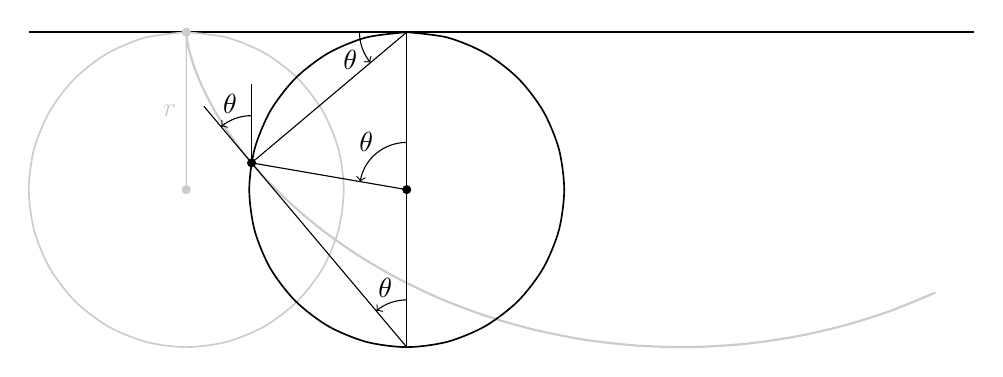
\begin{tikzpicture}
\pgfmathsetmacro{\r}{2.0}
\pgfmathsetmacro{\cangle}{0.7}   % current angle (psi)


% ceiling
\draw[thick] (-2, 0) -- (10,0);

% cycloid
\draw[thick, domain=0:2, smooth, variable=\t, color=black!20!white]
plot ({2*\t*\r - \r*sin(2*\t r)}, {-\r + \r*cos(2*\t r)});

% initial state, circle and radius
\draw[semithick, domain=0:3.141, smooth, variable=\t, color=black!20!white]
plot ({\r*sin(2*\t r)}, {-\r + \r*cos(2*\t r)});
\draw[color=black!20!white, fill=black!20!white] (0,0) circle[radius=0.05] -- node[left]{$r$} (0,-\r) circle[radius=0.05];

\coordinate (A) at ({2*\cangle*\r}, 0);   % contact point
\coordinate (B) at ({2*\cangle*\r}, {-\r});   % center of circle
\coordinate (C) at ({2*\cangle*\r}, {-2*\r});   % opposite point
\coordinate (D) at ({2*\cangle*\r - \r*sin(2*\cangle r)}, {-\r + \r*cos(2*\cangle r)});   % point on cycloid

% current state, circle and radius
\draw[semithick, domain=0:3.141, smooth, variable=\t]
plot ({2*\cangle*\r + \r*sin(2*\t r)}, {-\r + \r*cos(2*\t r)});
\draw[fill=black] (D) circle[radius=0.05] -- (B) circle[radius=0.05];

\draw (A) -- (C);
\draw (A) -- (D);
\draw (D) -- +(0,{0.5*\r});

\draw[->] (A)+({-0.3*\r},0) arc[start angle=180, end angle={180+deg(\cangle)}, radius={0.3*\r}];
\draw (A)+({pi r+0.65*\cangle r}:{0.4*\r}) node {$\theta$};

\draw[->] (B)+(0,{0.3*\r}) arc[start angle=90, end angle={90+deg(2*\cangle)}, radius={0.3*\r}];
\draw (B)+({pi/2 r+\cangle r}:{0.4*\r}) node {$\theta$};

\draw[->] (C)+(0,{0.3*\r}) arc[start angle=90, end angle={90+deg(\cangle)}, radius={0.3*\r}];
\draw (C)+({pi/2 r+\cangle/2 r}:{0.4*\r}) node {$\theta$};

\draw[->] (D)+(0,{0.3*\r}) arc[start angle=90, end angle={90+deg(\cangle)}, radius={0.3*\r}];
\draw (C) -- +({pi/2 r + \cangle r}:{2*\r});
\draw (D)+({pi/2 r+\cangle/2 r}:{0.4*\r}) node {$\theta$};

\end{tikzpicture}
 
